\documentclass[10pt,landscape]{article}
\usepackage[paperwidth=420mm,paperheight=297mm,margin=9mm]{geometry}
\usepackage[T1]{fontenc}
\usepackage[utf8]{inputenc}
\usepackage{tikz}
\usepackage{booktabs}
\usepackage{array}
\usepackage{xcolor}
\usepackage{amsmath}
\usepackage{hyperref}
\usetikzlibrary{arrows.meta,positioning,fit,calc,shapes.multipart}

\pagestyle{empty}
\setlength{\parindent}{0pt}
\renewcommand{\arraystretch}{1.15}

\definecolor{dataBlue}{RGB}{66,133,244}
\definecolor{condGreen}{RGB}{52,168,83}
\definecolor{diffOrange}{RGB}{245,124,0}
\definecolor{blockPurple}{RGB}{126,87,194}
\definecolor{lossRed}{RGB}{198,40,40}
\definecolor{grayBox}{RGB}{245,247,250}

\tikzset{
  tensor/.style={draw, rounded corners=2pt, very thick, fill=dataBlue!10, align=center, minimum height=9mm, font=\small},
  cond/.style={draw, rounded corners=2pt, very thick, fill=condGreen!10, align=center, minimum height=9mm, font=\small},
  op/.style={draw, rounded corners=2pt, very thick, fill=grayBox, align=center, minimum height=9mm, font=\small},
  unet/.style={draw, rounded corners=2pt, very thick, fill=diffOrange!12, align=center, minimum height=9mm, font=\small},
  block/.style={draw, rounded corners=2pt, very thick, fill=blockPurple!10, align=center, minimum height=9mm, font=\small},
  loss/.style={draw, rounded corners=2pt, very thick, fill=lossRed!8, align=center, minimum height=9mm, font=\small},
  arrow/.style={-{Latex[length=3mm]}, very thick},
  skip/.style={-{Latex[length=2.5mm]}, thick, dashed, color=blockPurple},
  note/.style={align=left, font=\footnotesize}
}

\newcommand{\shape}[1]{\texttt{[#1]}}
\newcommand{\cfg}{\texttt{dataset\_a\_256\_base48.yaml}}

\begin{document}

\begin{center}
{\Large Conditional Diffusion Network for Ultrasonic Defect Map Inversion}\\[1mm]
{\normalsize Main drawing follows \cfg: image size 256, pic channels 8, x channels 7, frequencies 15, base channels 48.}\\
{\small Tensor order: image tensors use \shape{B,C,H,W}; x-matrix uses \shape{B,C,F,TX,RX}.}
\end{center}

\vspace{1mm}

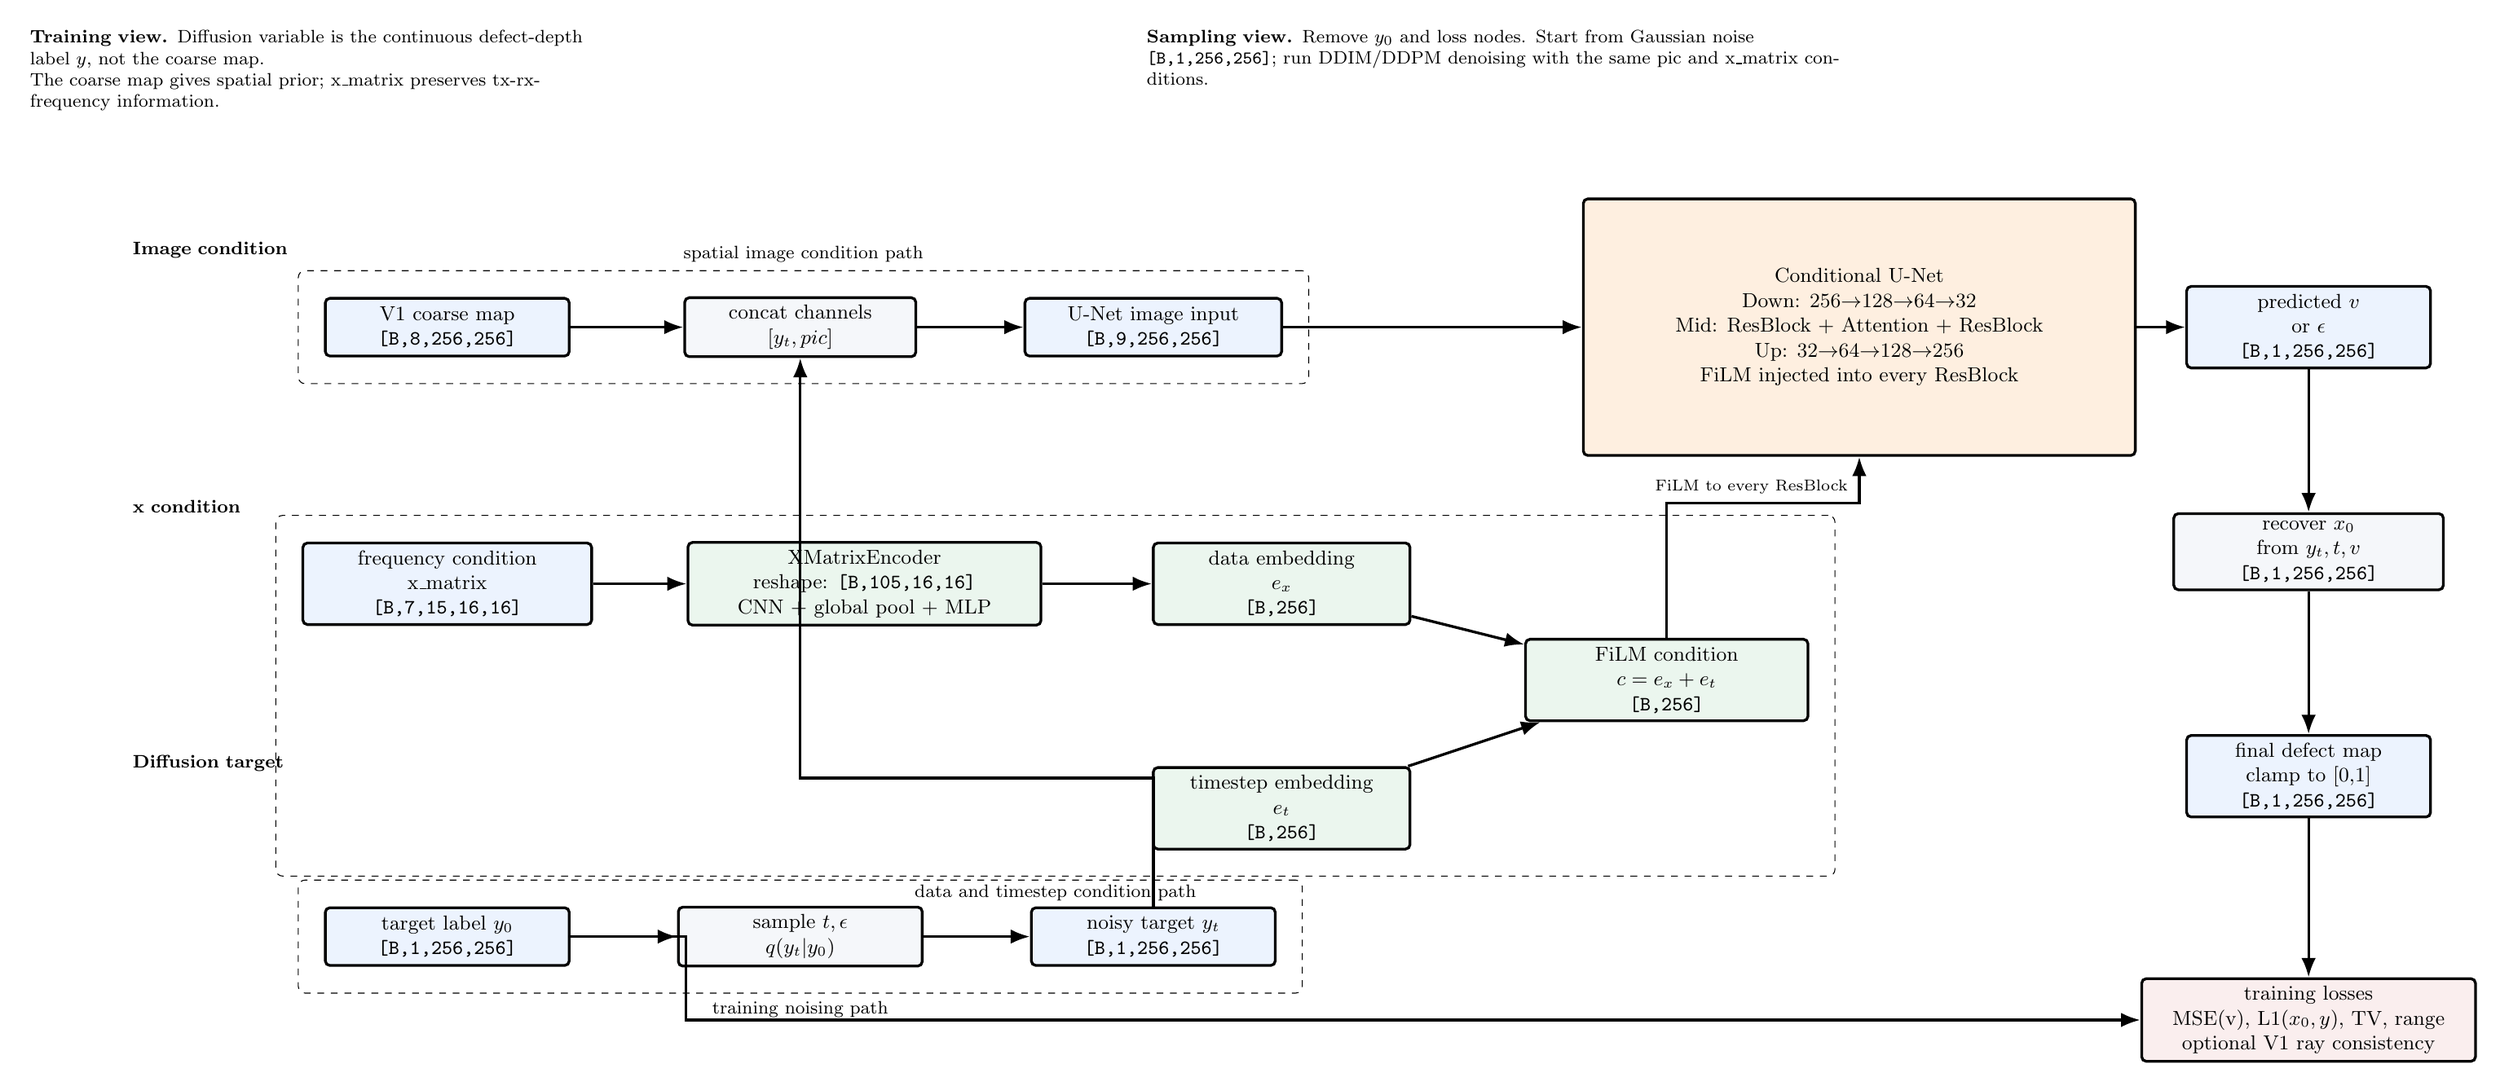
\begin{tikzpicture}[x=1mm,y=1mm]
  \node[note, text width=92mm] at (26,40) {
    \textbf{Training view.} Diffusion variable is the continuous defect-depth label $y$, not the coarse map.\\
    The coarse map gives spatial prior; x\_matrix preserves tx-rx-frequency information.
  };
  \node[note, text width=112mm] at (210,42) {
    \textbf{Sampling view.} Remove $y_0$ and loss nodes. Start from Gaussian noise \shape{B,1,256,256}; run DDIM/DDPM denoising with the same pic and x\_matrix conditions.
  };

  % Lane labels
  \node[note, text width=28mm] at (10,12) {\textbf{Image condition}};
  \node[note, text width=28mm] at (10,-28) {\textbf{x condition}};
  \node[note, text width=28mm] at (10,-68) {\textbf{Diffusion target}};

  % Image-condition lane
  \node[tensor, minimum width=38mm] (pic) at (45,0) {V1 coarse map\\\shape{B,8,256,256}};
  \node[op, minimum width=36mm] (concat) at (100,0) {concat channels\\$[y_t,pic]$};
  \node[tensor, minimum width=40mm] (unetin) at (155,0) {U-Net image input\\\shape{B,9,256,256}};

  % x-condition lane
  \node[tensor, minimum width=45mm] (xmat) at (45,-40) {frequency condition\\x\_matrix\\\shape{B,7,15,16,16}};
  \node[cond, minimum width=55mm] (xenc) at (110,-40) {XMatrixEncoder\\reshape: \shape{B,105,16,16}\\CNN + global pool + MLP};
  \node[cond, minimum width=40mm] (xemb) at (175,-40) {data embedding\\$e_x$\\\shape{B,256}};
  \node[cond, minimum width=40mm] (temb) at (175,-75) {timestep embedding\\$e_t$\\\shape{B,256}};
  \node[cond, minimum width=44mm] (film) at (235,-55) {FiLM condition\\$c=e_x+e_t$\\\shape{B,256}};

  % Diffusion-target lane
  \node[tensor, minimum width=38mm] (y0) at (45,-95) {target label $y_0$\\\shape{B,1,256,256}};
  \node[op, minimum width=38mm] (noise) at (100,-95) {sample $t,\epsilon$\\$q(y_t|y_0)$};
  \node[tensor, minimum width=38mm] (yt) at (155,-95) {noisy target $y_t$\\\shape{B,1,256,256}};

  % Main model and output stack
  \node[unet, minimum width=86mm, minimum height=40mm] (unetbox) at (265,0) {
    Conditional U-Net\\
    Down: 256$\rightarrow$128$\rightarrow$64$\rightarrow$32\\
    Mid: ResBlock + Attention + ResBlock\\
    Up: 32$\rightarrow$64$\rightarrow$128$\rightarrow$256\\
    FiLM injected into every ResBlock
  };
  \node[tensor, minimum width=38mm] (vpred) at (335,0) {predicted $v$\\or $\epsilon$\\\shape{B,1,256,256}};
  \node[op, minimum width=42mm] (x0pred) at (335,-35) {recover $x_0$\\from $y_t,t,v$\\\shape{B,1,256,256}};
  \node[tensor, minimum width=38mm] (out) at (335,-70) {final defect map\\clamp to [0,1]\\\shape{B,1,256,256}};
  \node[loss, minimum width=52mm] (losses) at (335,-108) {training losses\\MSE(v), L1($x_0,y$), TV, range\\optional V1 ray consistency};

  % Straight lane arrows
  \draw[arrow] (pic) -- (concat);
  \draw[arrow] (concat) -- (unetin);
  \draw[arrow] (unetin) -- (unetbox);
  \draw[arrow] (xmat) -- (xenc);
  \draw[arrow] (xenc) -- (xemb);
  \draw[arrow] (xemb) -- (film);
  \draw[arrow] (temb) -- (film);
  \draw[arrow] (y0) -- (noise);
  \draw[arrow] (noise) -- (yt);
  \draw[arrow] (unetbox) -- (vpred);
  \draw[arrow] (vpred) -- (x0pred);
  \draw[arrow] (x0pred) -- (out);
  \draw[arrow] (out) -- (losses);

  % Routed arrows that avoid node text
  \draw[arrow] (yt.north) -- ++(0,20) -| (concat.south);
  \draw[arrow] (film.north) -- ++(0,21) -| node[pos=0.22,above,font=\scriptsize]{FiLM to every ResBlock} (unetbox.south);
  \draw[arrow] (y0.east) -- ++(18,0) |- (losses.west);

  % Visual grouping
  \node[draw, rounded corners=3pt, dashed, fit=(pic)(concat)(unetin), inner sep=4mm, label={[font=\footnotesize]above:spatial image condition path}] {};
  \node[draw, rounded corners=3pt, dashed, fit=(xmat)(xenc)(xemb)(temb)(film), inner sep=4mm, label={[font=\footnotesize]below:data and timestep condition path}] {};
  \node[draw, rounded corners=3pt, dashed, fit=(y0)(noise)(yt), inner sep=4mm, label={[font=\footnotesize]below:training noising path}] {};
\end{tikzpicture}

\newpage

\begin{center}
{\Large U-Net Tensor Shapes and Block Counts}\\[1mm]
{\small Configuration: base=48, channel\_mult=[1,2,4,4], num\_res\_blocks=2, attention\_resolutions=[32].}
\end{center}

\begin{tabular}{>{\raggedright\arraybackslash}p{28mm} >{\raggedright\arraybackslash}p{43mm} >{\raggedright\arraybackslash}p{38mm} >{\raggedright\arraybackslash}p{42mm} >{\raggedright\arraybackslash}p{90mm}}
\toprule
Stage & Operation & Input shape & Output shape & Notes \\
\midrule
Input concat & concat $y_t$ and pic & \shape{B,1,256,256} + \shape{B,8,256,256} & \shape{B,9,256,256} & image condition is channel-concatenated. \\
Input conv & 3x3 conv & \shape{B,9,256,256} & \shape{B,48,256,256} & first feature map. \\
Down level 0 & 2 x ResBlock(48) & \shape{B,48,256,256} & \shape{B,48,256,256} & stores 2 skip tensors at 256. \\
Downsample 0 & stride-2 conv & \shape{B,48,256,256} & \shape{B,48,128,128} & stores pre-downsample skip. \\
Down level 1 & ResBlock 48->96, ResBlock 96->96 & \shape{B,48,128,128} & \shape{B,96,128,128} & stores 2 skip tensors at 128. \\
Downsample 1 & stride-2 conv & \shape{B,96,128,128} & \shape{B,96,64,64} & stores pre-downsample skip. \\
Down level 2 & ResBlock 96->192, ResBlock 192->192 & \shape{B,96,64,64} & \shape{B,192,64,64} & stores 2 skip tensors at 64. \\
Downsample 2 & stride-2 conv & \shape{B,192,64,64} & \shape{B,192,32,32} & stores pre-downsample skip. \\
Down level 3 & 2 x ResBlock(192) + Attention after each & \shape{B,192,32,32} & \shape{B,192,32,32} & stores 2 skip tensors at 32. \\
Middle & ResBlock + Attention + ResBlock & \shape{B,192,32,32} & \shape{B,192,32,32} & bottleneck. \\
Up level 3 & 2 x concat skip + ResBlock(384->192) + Attention & \shape{B,192,32,32} & \shape{B,192,32,32} & consumes two 32 skips. \\
Upsample 3 & nearest upsample + 3x3 conv & \shape{B,192,32,32} & \shape{B,192,64,64} & moves to 64. \\
Up level 2 & 3 x concat skip + ResBlock & \shape{B,192,64,64} & \shape{B,192,64,64} & consumes downsample skip + two 64 skips. \\
Upsample 2 & nearest upsample + 3x3 conv & \shape{B,192,64,64} & \shape{B,192,128,128} & moves to 128. \\
Up level 1 & 3 x concat skip + ResBlock & \shape{B,192,128,128} & \shape{B,96,128,128} & final channel count at this level is 96. \\
Upsample 1 & nearest upsample + 3x3 conv & \shape{B,96,128,128} & \shape{B,96,256,256} & moves to 256. \\
Up level 0 & 3 x concat skip + ResBlock & \shape{B,96,256,256} & \shape{B,48,256,256} & final high-res feature map. \\
Output head & GroupNorm + SiLU + 3x3 conv & \shape{B,48,256,256} & \shape{B,1,256,256} & predicts $v$ by default. \\
\bottomrule
\end{tabular}

\vspace{4mm}

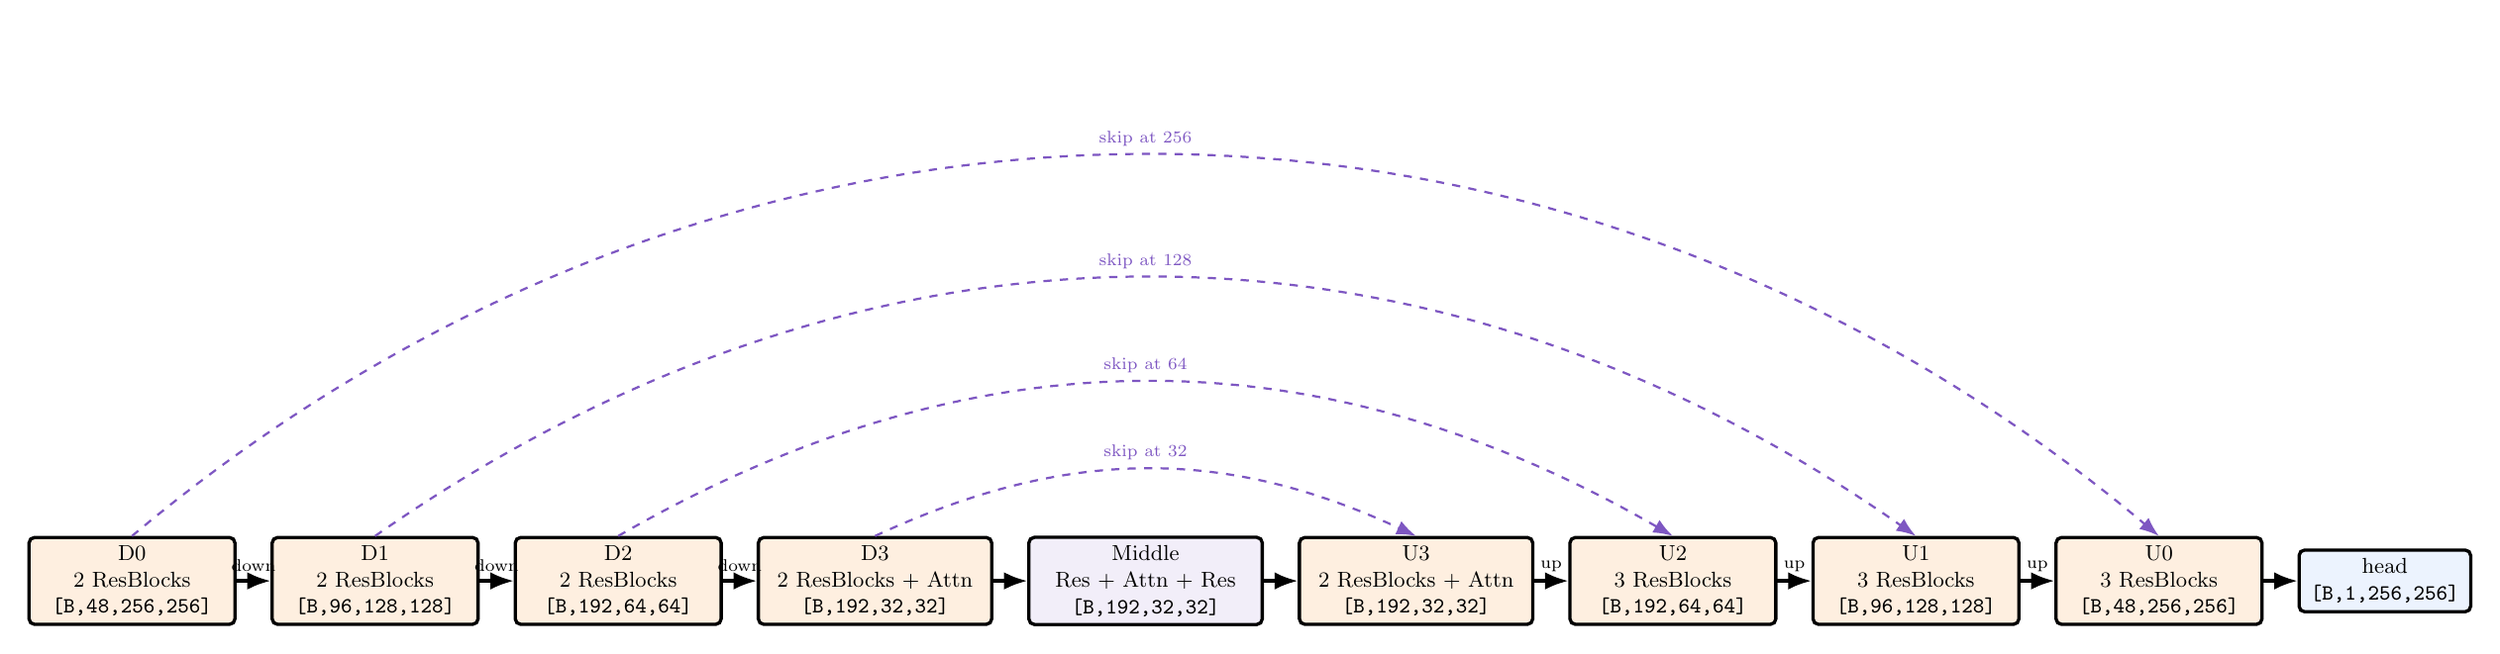
\begin{tikzpicture}[node distance=6mm and 5mm, transform shape, scale=0.88]
  \node[unet, minimum width=30mm] (d0) {D0\\2 ResBlocks\\\shape{B,48,256,256}};
  \node[unet, minimum width=30mm, right=of d0] (d1) {D1\\2 ResBlocks\\\shape{B,96,128,128}};
  \node[unet, minimum width=30mm, right=of d1] (d2) {D2\\2 ResBlocks\\\shape{B,192,64,64}};
  \node[unet, minimum width=34mm, right=of d2] (d3) {D3\\2 ResBlocks + Attn\\\shape{B,192,32,32}};
  \node[block, minimum width=34mm, right=of d3] (mid) {Middle\\Res + Attn + Res\\\shape{B,192,32,32}};
  \node[unet, minimum width=34mm, right=of mid] (u3) {U3\\2 ResBlocks + Attn\\\shape{B,192,32,32}};
  \node[unet, minimum width=30mm, right=of u3] (u2) {U2\\3 ResBlocks\\\shape{B,192,64,64}};
  \node[unet, minimum width=30mm, right=of u2] (u1) {U1\\3 ResBlocks\\\shape{B,96,128,128}};
  \node[unet, minimum width=30mm, right=of u1] (u0) {U0\\3 ResBlocks\\\shape{B,48,256,256}};
  \node[tensor, minimum width=25mm, right=of u0] (head) {head\\\shape{B,1,256,256}};

  \draw[arrow] (d0) -- node[above,font=\scriptsize]{down} (d1);
  \draw[arrow] (d1) -- node[above,font=\scriptsize]{down} (d2);
  \draw[arrow] (d2) -- node[above,font=\scriptsize]{down} (d3);
  \draw[arrow] (d3) -- (mid);
  \draw[arrow] (mid) -- (u3);
  \draw[arrow] (u3) -- node[above,font=\scriptsize]{up} (u2);
  \draw[arrow] (u2) -- node[above,font=\scriptsize]{up} (u1);
  \draw[arrow] (u1) -- node[above,font=\scriptsize]{up} (u0);
  \draw[arrow] (u0) -- (head);

  \draw[skip] (d3.north) to[bend left=25] node[above,font=\scriptsize]{skip at 32} (u3.north);
  \draw[skip] (d2.north) to[bend left=30] node[above,font=\scriptsize]{skip at 64} (u2.north);
  \draw[skip] (d1.north) to[bend left=35] node[above,font=\scriptsize]{skip at 128} (u1.north);
  \draw[skip] (d0.north) to[bend left=40] node[above,font=\scriptsize]{skip at 256} (u0.north);
\end{tikzpicture}

\newpage

\begin{center}
{\Large Block Internal Structure}
\end{center}

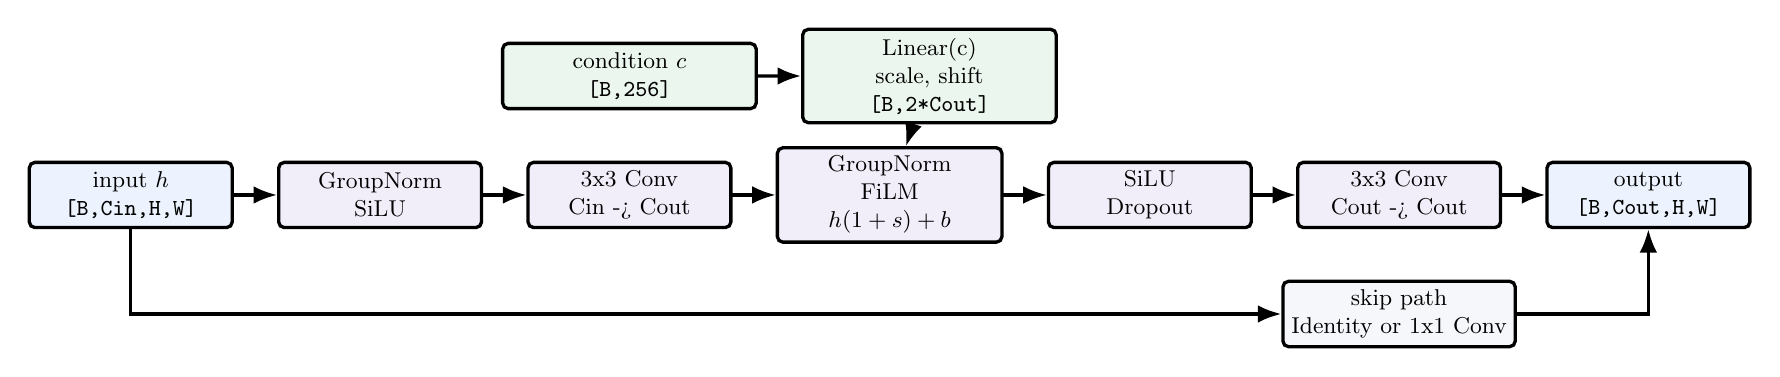
\begin{tikzpicture}[node distance=7mm and 6mm, transform shape, scale=0.92]
  \node[tensor, minimum width=28mm] (xin) {input $h$\\\shape{B,Cin,H,W}};
  \node[block, minimum width=28mm, right=of xin] (gn1) {GroupNorm\\SiLU};
  \node[block, minimum width=28mm, right=of gn1] (conv1) {3x3 Conv\\Cin -> Cout};
  \node[cond, minimum width=35mm, above=of conv1] (cond) {condition $c$\\\shape{B,256}};
  \node[cond, minimum width=35mm, right=of cond] (lin) {Linear(c)\\scale, shift\\\shape{B,2*Cout}};
  \node[block, minimum width=31mm, right=of conv1] (gn2) {GroupNorm\\FiLM\\$h(1+s)+b$};
  \node[block, minimum width=28mm, right=of gn2] (drop) {SiLU\\Dropout};
  \node[block, minimum width=28mm, right=of drop] (conv2) {3x3 Conv\\Cout -> Cout};
  \node[op, minimum width=28mm, below=of conv2] (skip) {skip path\\Identity or 1x1 Conv};
  \node[tensor, minimum width=28mm, right=of conv2] (xout) {output\\\shape{B,Cout,H,W}};

  \draw[arrow] (xin) -- (gn1);
  \draw[arrow] (gn1) -- (conv1);
  \draw[arrow] (conv1) -- (gn2);
  \draw[arrow] (gn2) -- (drop);
  \draw[arrow] (drop) -- (conv2);
  \draw[arrow] (conv2) -- (xout);
  \draw[arrow] (xin) |- (skip);
  \draw[arrow] (skip) -| (xout);
  \draw[arrow] (cond) -- (lin);
  \draw[arrow] (lin) -- (gn2);
\end{tikzpicture}

\vspace{6mm}

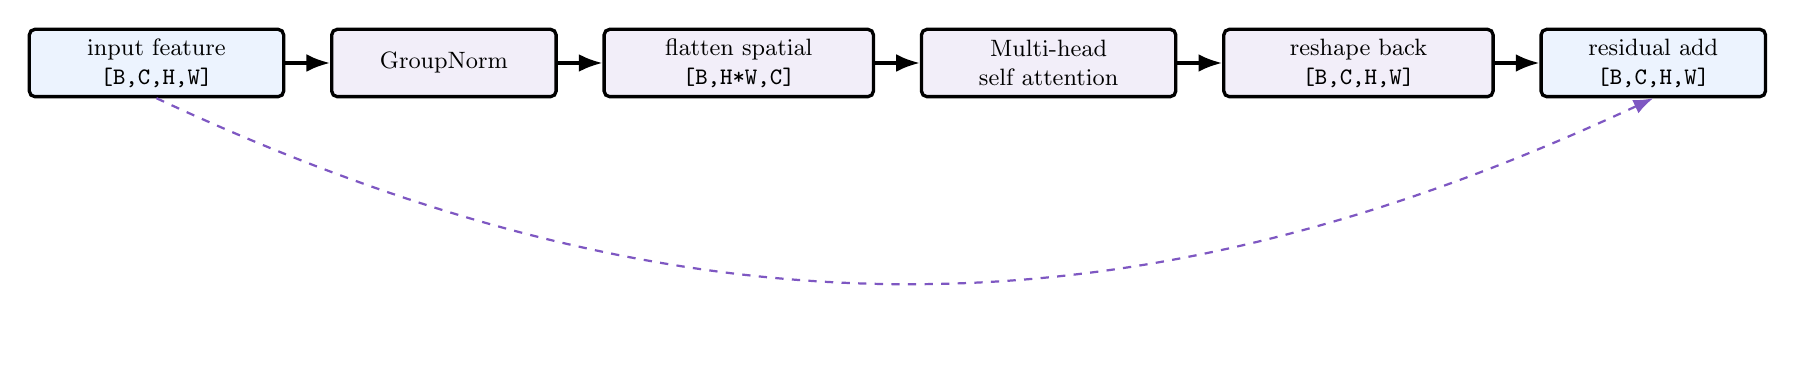
\begin{tikzpicture}[node distance=7mm and 6mm, transform shape, scale=0.95]
  \node[tensor, minimum width=34mm] (ain) {input feature\\\shape{B,C,H,W}};
  \node[block, minimum width=30mm, right=of ain] (norm) {GroupNorm};
  \node[block, minimum width=36mm, right=of norm] (flat) {flatten spatial\\\shape{B,H*W,C}};
  \node[block, minimum width=34mm, right=of flat] (mha) {Multi-head\\self attention};
  \node[block, minimum width=36mm, right=of mha] (unflat) {reshape back\\\shape{B,C,H,W}};
  \node[tensor, minimum width=30mm, right=of unflat] (aout) {residual add\\\shape{B,C,H,W}};

  \draw[arrow] (ain) -- (norm);
  \draw[arrow] (norm) -- (flat);
  \draw[arrow] (flat) -- (mha);
  \draw[arrow] (mha) -- (unflat);
  \draw[arrow] (unflat) -- (aout);
  \draw[skip] (ain.south) to[bend right=25] (aout.south);
\end{tikzpicture}

\vspace{6mm}

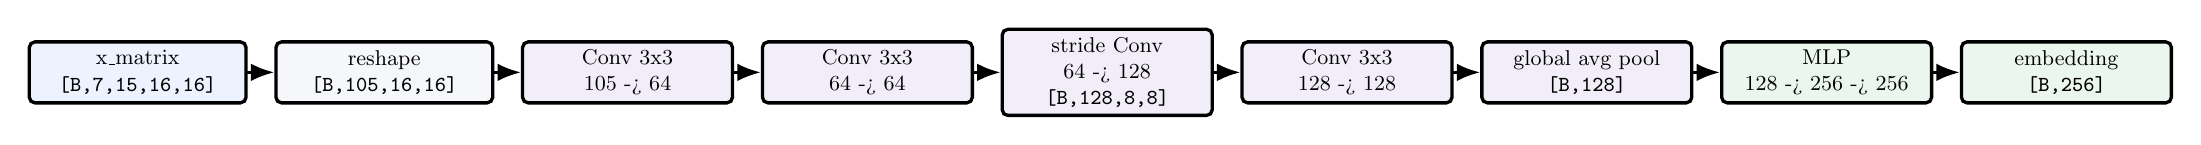
\begin{tikzpicture}[node distance=6mm and 4mm, transform shape, scale=0.86]
  \node[tensor, minimum width=32mm] (xm) {x\_matrix\\\shape{B,7,15,16,16}};
  \node[op, minimum width=32mm, right=of xm] (reshape) {reshape\\\shape{B,105,16,16}};
  \node[block, minimum width=31mm, right=of reshape] (c1) {Conv 3x3\\105 -> 64};
  \node[block, minimum width=31mm, right=of c1] (c2) {Conv 3x3\\64 -> 64};
  \node[block, minimum width=31mm, right=of c2] (c3) {stride Conv\\64 -> 128\\\shape{B,128,8,8}};
  \node[block, minimum width=31mm, right=of c3] (c4) {Conv 3x3\\128 -> 128};
  \node[block, minimum width=31mm, right=of c4] (pool) {global avg pool\\\shape{B,128}};
  \node[cond, minimum width=31mm, right=of pool] (mlp) {MLP\\128 -> 256 -> 256};
  \node[cond, minimum width=31mm, right=of mlp] (emb) {embedding\\\shape{B,256}};

  \draw[arrow] (xm) -- (reshape);
  \draw[arrow] (reshape) -- (c1);
  \draw[arrow] (c1) -- (c2);
  \draw[arrow] (c2) -- (c3);
  \draw[arrow] (c3) -- (c4);
  \draw[arrow] (c4) -- (pool);
  \draw[arrow] (pool) -- (mlp);
  \draw[arrow] (mlp) -- (emb);
\end{tikzpicture}

\vspace{4mm}

\begin{tabular}{>{\raggedright\arraybackslash}p{45mm} >{\raggedright\arraybackslash}p{205mm}}
\toprule
Block & Stack rule in code \\
\midrule
ResBlock & GroupNorm + SiLU + Conv, then FiLM-conditioned GroupNorm, SiLU + Dropout + Conv, plus identity or 1x1 skip. Every ResBlock receives the same condition vector $c=e_x+e_t$. \\
AttentionBlock & Used only where spatial resolution equals 32 for base48 config. It is self-attention over the flattened $H \times W$ locations. \\
Downsample & 3x3 stride-2 convolution. Channels stay the same; resolution halves. \\
Upsample & nearest-neighbor upsample by 2, then 3x3 convolution. Channels stay the same; resolution doubles. \\
Skip concatenation & Decoder ResBlocks concatenate the current feature with the latest saved encoder skip tensor along the channel dimension before the ResBlock. \\
\bottomrule
\end{tabular}

\newpage

\begin{center}
{\Large Diffusion Training and Sampling Equations}
\end{center}

\begin{tabular}{>{\raggedright\arraybackslash}p{45mm} >{\raggedright\arraybackslash}p{205mm}}
\toprule
Step & Formula and tensor shape \\
\midrule
Forward noising & $y_t=\sqrt{\bar{\alpha}_t}y_0+\sqrt{1-\bar{\alpha}_t}\epsilon$, all image tensors are \shape{B,1,256,256}. \\
Condition image & $\mathrm{input}=\mathrm{concat}(y_t, pic)$ gives \shape{B,9,256,256}. \\
Condition vector & $e_x=\mathrm{XMatrixEncoder}(x)$, $e_t=\mathrm{TimeEmbedding}(t)$, $c=e_x+e_t$, all \shape{B,256}. \\
Network prediction & $\hat{v}=\mathrm{ConditionalUNet}([y_t,pic],t,e_x)$ with shape \shape{B,1,256,256}. \\
Training target & With \texttt{prediction\_type=v\_prediction}: $v=\sqrt{\bar{\alpha}_t}\epsilon-\sqrt{1-\bar{\alpha}_t}y_0$. \\
Main loss & $L_{diff}=\mathrm{MSE}(\hat{v},v)$. \\
Auxiliary clean prediction & $\hat{x}_0=\sqrt{\bar{\alpha}_t}y_t-\sqrt{1-\bar{\alpha}_t}\hat{v}$, then use L1/TV/range/optional physics losses. \\
Sampling & Start from $y_T\sim\mathcal{N}(0,I)$ and run DDIM/DDPM reverse steps with the same pic and x\_matrix conditions. Final output is clamped to \shape{B,1,256,256}. \\
\bottomrule
\end{tabular}

\vspace{5mm}

\begin{tabular}{>{\raggedright\arraybackslash}p{55mm} >{\raggedright\arraybackslash}p{195mm}}
\toprule
Configuration note & Meaning \\
\midrule
This PDF main architecture & Uses \texttt{dataset\_a\_256\_base48.yaml}. This is the recommended 256 first-version model in the code. \\
Debug config difference & \texttt{dataset\_a\_256\_debug.yaml} uses base=32, channel\_mult=[1,2,4], num\_res\_blocks=1, cond\_dim=192. Its path is the same but shorter: 256 -> 128 -> 64 bottleneck instead of 256 -> 128 -> 64 -> 32. \\
Base64 config difference & \texttt{dataset\_a\_256\_base64.yaml} keeps the same topology as base48 but increases base channels to 64. Channel sequence becomes 64,128,256,256. \\
\bottomrule
\end{tabular}

\end{document}
